\chapter{Conducted Measurements} \label{chap:5}

The term Conducted Measurements refers to measurements performed using \acs{RF} cables connected between the antenna of the \acs{DUT} and the instruments (off-air). Most \acs{WLAN} regulatory compliance mandate that conducted measurements shall be used for most compliance tests (transmit power, in-band spectrum density, bandwidth, and parts of the spurious scan) for a \acs{DUT} with antenna connector(s) and using a dedicated external antenna(s), or for a \acs{DUT} with integrated antenna(s) but with temporary antenna connector(s) provided. As mentioned in the chapter \ref{chap:test}, this thesis implements tests for \acf{OBW} measurement, \acf{PSD} measurement, and \acf{RxBlocking} Measurement.

\section{Using Attenuator and Splitter}
\label{sec:att}
Figures \ref{fig:Ng1} and \ref{fig:Ng2} show the block diagram of the connections of the instruments during conducted measurements. To not complicate things, the \acs{DUT} is connected via a Wi-Fi connection to a laptop. The \acs{DUT} in this case is a single antenna \acs{DUT} (Archer T2UH \ref{fig:singleAntennaDUT}). This DUT is further associated with the \ac{CMW} (wireless connectivity tester). The companion device acts as an access point. The splitter is used to split a single acs{RF} line into two different \acs{RF} lines. The attenuator of 20 dB is required to reduce the signal strength. When using a spectrum analyzer, the attenuator benefits by not allowing the spectrum analyzer to measure the power coming from the companion device. The dark blue lines in the figure indicate a strong signal in the direction while the light blue line shows the weaker signals. \\

\begin{figure}[H]
\centering
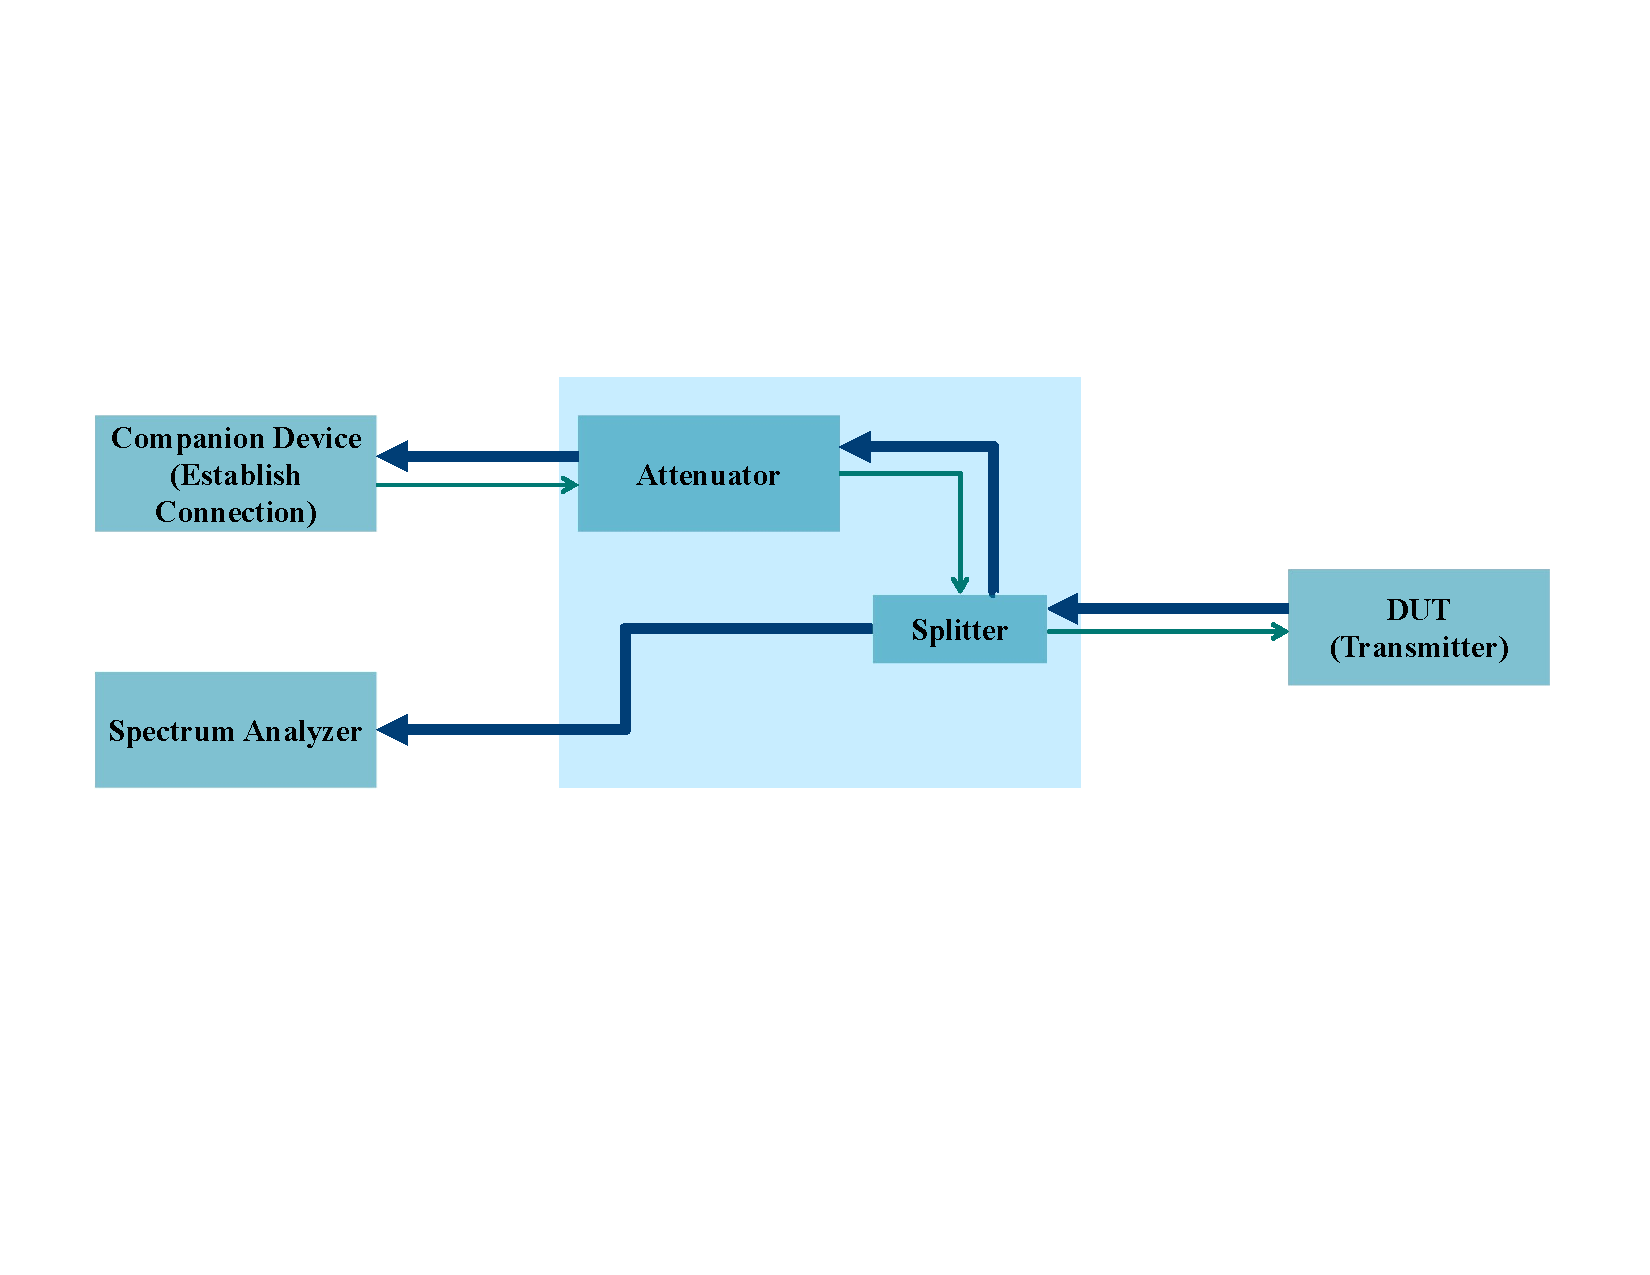
\includegraphics[width=0.65\textwidth]{conductedtx.pdf}
 \caption{Conducted measurements using attenuators and splitters: \acs{DUT} behaves as a transmitter}
 \label{fig:Ng1} 
\end{figure}

\begin{figure}[H]
\centering
   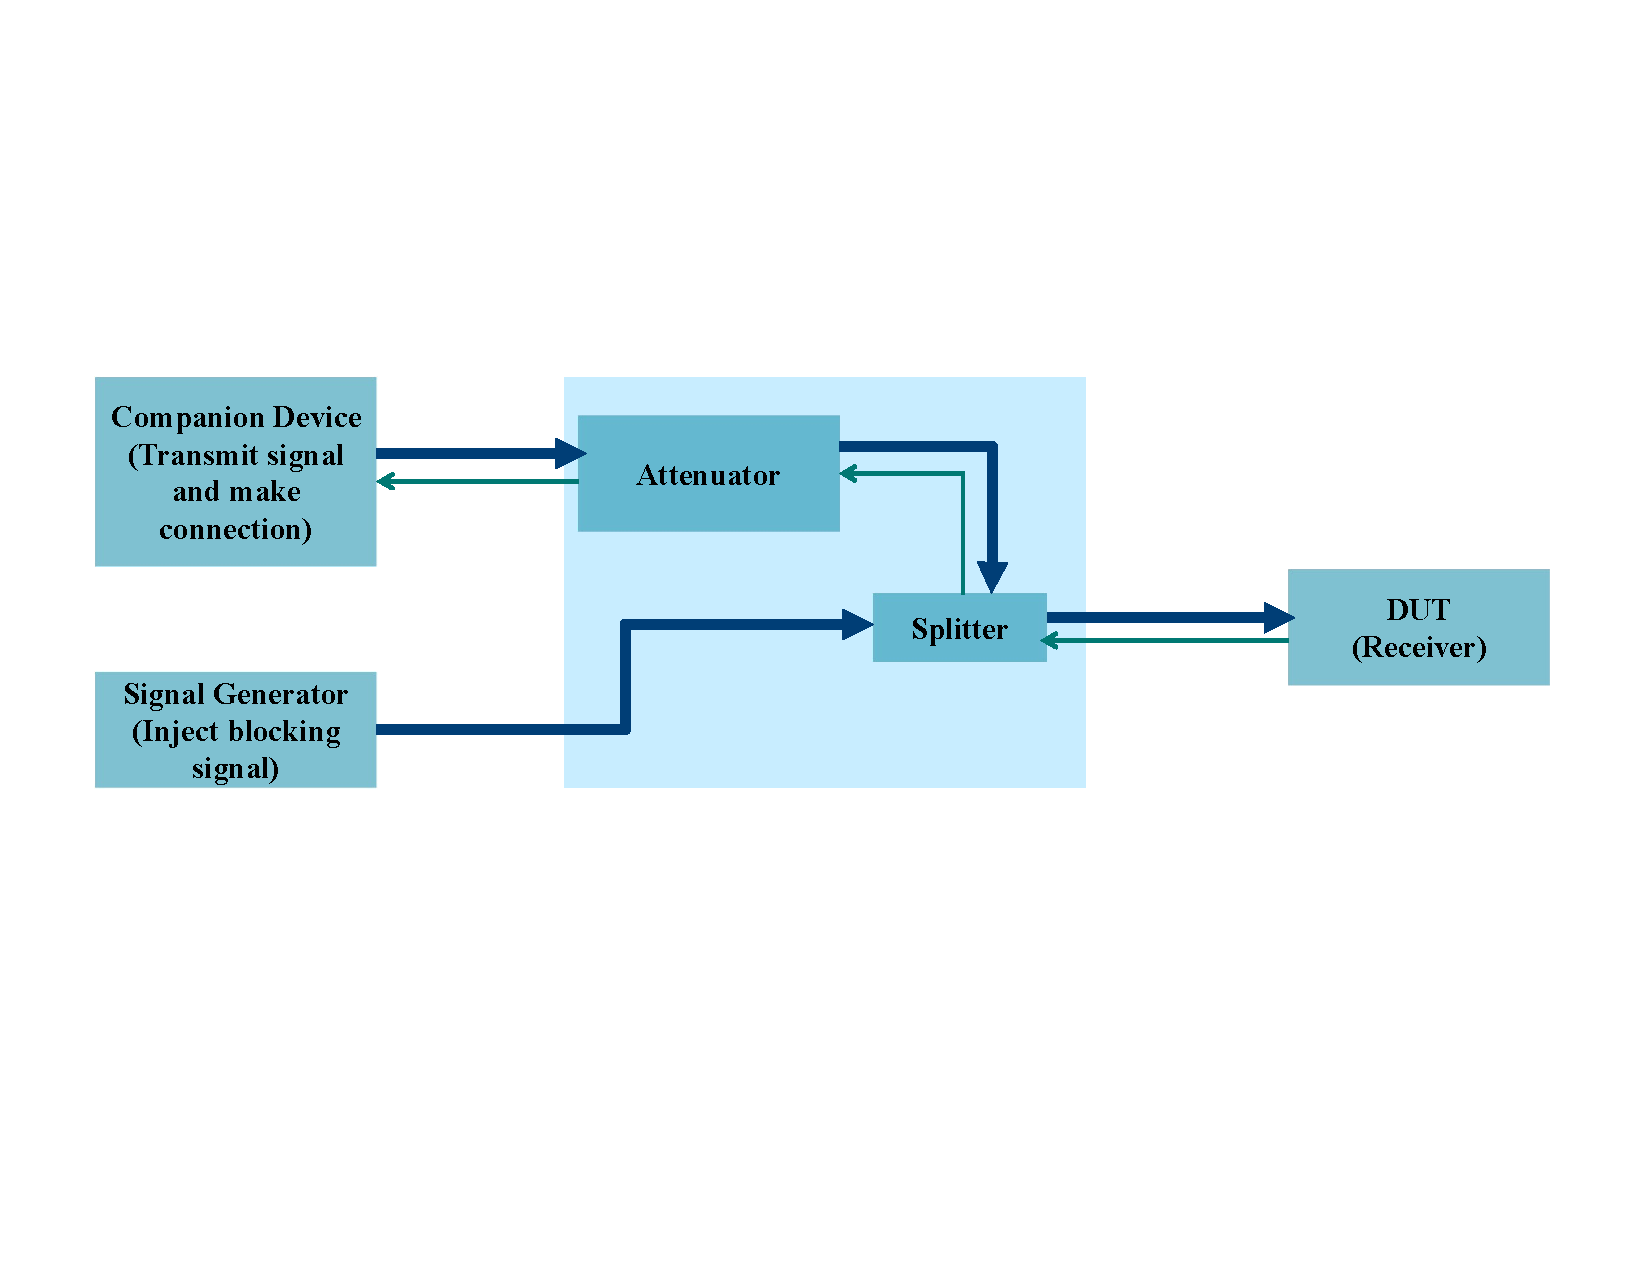
\includegraphics[width=0.65\textwidth]{conductedrx.pdf}
   \caption{Conducted measurements using attenuators and splitters: \acs{DUT} behaves as a receiver}
   \label{fig:Ng2}
\end{figure}

The hardware setup shown in Figure \ref{fig:Ng1} performs the \acf{OBW} and \acf{PSD} measurement. The spectrum analyzer is used to measure the spectrum of the signal from the \acs{DUT} and then assess the \acf{OBW} or the \acf{PSD} based on this data. Since the \acs{DUT} behaves like a transmitter, most of the signal is going away from the \acs{DUT} (dark blue lines) but there is also some receiving when a connection is established between the \acf{CMW} and the \acs{DUT}. The approach to find 99\% of the\acf{OBW} and \acf{PSD} is explained in the section \ref{sec:obw}.\\

When the \acs{DUT} acts as a receiver in Figure \ref{fig:Ng2}, the signal generator generates a blocking signal (unwanted signal) on the frequencies other than those of the operating band.  \acf{PER} measurement examines the ability of the \acs{DUT} to receive a wanted signal on its operating channel without exceeding 10\% degradation in the presence of a blocking signal. 

\section{Using a Switching Matrix}
\label{sec:switch}
The next goal is to use a dedicated switching matrix instead of changing splitters and attenuators for every test measurement. Before starting the measurement, the first step is to switch the correct paths within the switching modules required for the test. \\

For the receiver blocking test case, the blocker power level at the signal generator is calculated by adding the cable losses, attenuation from the switching units, and the antenna gain of the \acs{DUT} to the blocker power level mentioned in the standard. The formula to calculate the blocker level at the generator is shown in equation \ref{eq:1}:

\begin{equation}
\begin{aligned}
\mbox{Blocker level}_ {\mbox{Gen}} = &\mbox{Required blocker level in front of the DUT} \\
&+ \mbox{Attenuation}_{\mbox{cables}} \\
&+ \mbox{Attenuation}_{\mbox{switchingUnits}}  \\
&+ \mbox{Antenna Gain}_{\mbox{ DUT}}
\label{eq:1}
\end{aligned}
\end{equation}

For example, the standard mentions that at blocker frequency of 2360 MHz, the required blocker level in front of the DUT is -53 dBm. Assume the total attenuation is 40 dB and the antenna gain of the DUT is 3 dBi. Then,
$$\mbox{Blocker Level at the Generator} = -53 \mbox{dBm} + 40 \mbox{dB}+ 3 \mbox{dBi} = -10 \mbox{dBm}$$ \\

(\textbf{diagram})\\

The results from \acf{RxBlocking} and \acf{OBW} measurements are compared with the implementation in the WMS32 software suite. The results match and therefore the next step is to perform normalized measurements, which is explained in the chapter \ref{chap:normalized}.






